\chapter{行波管的构造和工作原理}
\section{行波管的构造}
我们来看一只微波通信中常用的中小功率行波管,这类行波管都采用螺旋线来作为它的慢波系统,因此又叫做螺旋线型行波管,图\ref{ch2-1}是它的基本结构图。图\ref{ch2-2}则是其各电极的电源接线图。由图可见,行波管和双腔速调管一样,都有阴极、聚束极、加速极和收集极。不同的地方就在于:我们在行波管中用慢波系统(螺旋线)代替了速调管中的谐振腔和漂移管。这样一来,输能装置也发生了相应的变化。关于行波管中采用慢波系统的原因,我们将在后面讲到。

\begin{figure}[phtb]
	\centering
	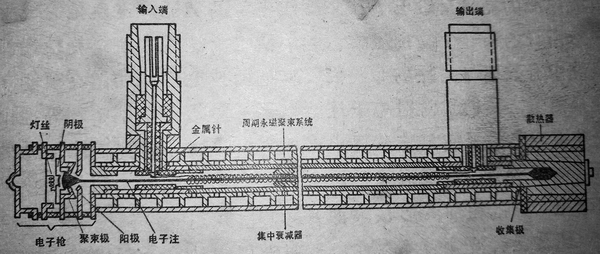
\includegraphics[width=\linewidth]{figure/ch2-1}
	\caption{行波管基本结构示意图}
	\label{ch2-1}
\end{figure}

\begin{figure}[phtb]
	\centering
	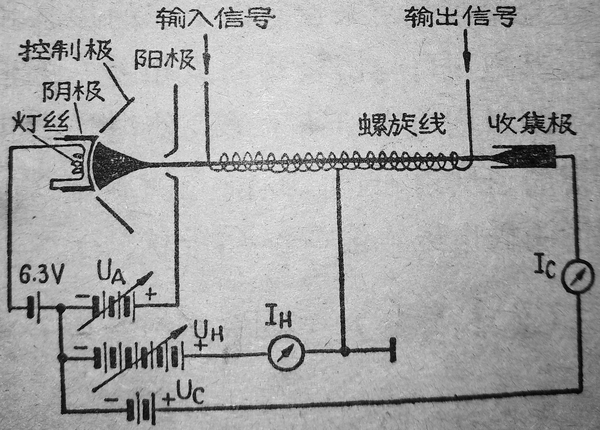
\includegraphics[width=0.65\linewidth]{figure/ch2-2}
	\caption{行波管各极电源接线图}
	\label{ch2-2}
\end{figure}

通常,一只行波管由五部分组成:
\subsection{电子枪}
电子枪通常由阴极、聚束极和加速极(即阳极)组成。它的任务是产生一束具有一定能量的高速细束电子流(常叫做电子注或电子束)。从能量关系来看,电子枪所做的工作就是把直流电源的能量交给电子注,变成电子的动能,也就是完成上一章所说的第一个物理过程。为了使电子注能够在螺旋线慢波系统中有效的与高频场(我们习惯把微波电磁场叫做高频场)交换能量,我们常常对电子注的直径、形状、电流密度等提出一些要求。为了满足这些要求,就需要在电子枪里面增加一些新的电极,例如聚束极就是。电子枪中各个电极的形状和电压,对于电子注的粗细、形状等都有影响。

阴极是行波管的“心脏”,通常用镍的合金制成,发射面做成凹球面状,其表面涂敷一层发射电子的活性物质。

聚束极是用来控制电子注的形状和粗细的,常做成漏斗状,其电压可与阴极相同或相差(低于或高于)几十伏。

阳极则用来加速电子,使电子离开阴极穿过阳极小孔后以一定的速度射入慢波系统(螺旋线)。对中小功率行波管来说,阳极电压一般是2—3千伏。
\subsection{信号输入、输出耦合装置(或输能装置)}
常见的有同轴和波导两种形式,图2-1所示的耦合装置为同轴形式,其内导体与金属针上端接触,金属针下端,则在管内与螺旋线的端部焊牢。同轴接头的外导体与金属管壳相接触。需要放大的高频信号(我们习惯把微波信号叫做高频信号,因而把行波管中与微波信号有关的部分称为高频部分或高频结构。通常我们所说的高频结构,主要就是指慢波系统)由输入装置送入管内,放大后的信号则由输出装置输出。
\subsection{螺旋线慢波系统}
它被用来降低高频场沿管轴的传播速度,使之与电子注的速度相近,以便与电子注进行充分的能量交换,完成把电子的动能转换成高频场能量这一物理过程(详见第三章)。
\subsection{收集极和散热器}
在慢波系统中完成了能量转换任务的电子注穿出螺旋线后被收集极所收集。由于电子注的速度很高,因此收集的热损耗很大,为防止收集极温度过高而损坏行波管,通常在收集外面装有散热器,使能量有效地散出去(详见第八章)。
\subsection{磁聚束系统(磁聚焦系统)}
螺旋线的内径通常只有2—3毫米,电子注的直径就更小,在这样细的电子注内,电子之间的相互排斥力(即所谓空间电荷斥力)很大。因此,要使电子注顺利地穿过长达一、二百毫米以上的螺旋线是十分困难的。为了克服这个困难,我们常常采用外加轴向磁场的办法来限制电子注的向外发散,使他能保持一定的粗细,顺利地穿过螺旋线。这个轴向磁场系统便称为磁聚束系统,它也是行波管中很重要的一部分(详见第七章)。

以上介绍的是行波管必须具备的五个基本组成部分,下面让我们看看行波管是怎样放大微波信号的。
\section{行波管放大的基本原理}
\subsection{双腔速调管的频带为什么那么窄?}
双腔速调管的频带之所以比较窄,其根源就在那个“腔”上。我们知道,谐振腔就是微波频率下的振荡回路,只有谐振频率附近的信号,才能够在谐振腔内建立起高频电场,而非谐振频率(离谐振频率较远)的信号就不能在谐振腔内建立起高频电场。因此,当非谐振频率的信号输入到双腔速调管内时,就不能在谐振腔隙缝处,建立起高频电场,因而不能对电子注进行速度调制,当然密度调制也就无从谈起了。可见正是谐振腔这个窄频带元件限制了双腔速调管的工作频带。因此,为了增宽工作频带,就不能采用谐振腔这样的元件。不过在取消谐振腔之前,我们应该搞清楚谐振腔在双腔速调管中所起的作用、它有哪些特点等,这将有助于我们寻找新的能量作用元件。

在双腔速调管中,谐振腔是电子与高频电场进行能量相互作用的场所。由于谐振腔内的高频电场高度集中在栅网隙缝处,那儿的高频电场就特别强,因此,当交变电子流穿过隙缝时,虽然时间非常短,但是它们之间的相互作用是十分强烈的。于是,我们便能在输出腔得到很强的输出信号,达到放大微波信号的目的。可见,谐振腔的特点是:电场集中,与电子流相互作用强烈,但作用时间很短。谐振腔的这个特点是与他是一个驻波型元件分不开的。我们知道,驻波型元件的能量都比较集中,它占有的空间比较小,但频带都比较窄。

看来为了展宽频带,我们不能再用驻波型元件了。于是,人们提出了一个新的想法——采用行波型元件,具体说来就是传输线。传输线在匹配良好的条件下,它的频带是比较宽的。但是,在传输线中,能量是沿传输线不断向前传播的,不像谐振腔隙缝中那样集中,因而与电子流的相互作用也就比较弱。怎样来克服这个缺点呢?我们采取了“因势利导”的办法:既然高频电磁场要沿着传输线不断地向前传播,那么我们能不能让电子流也跟着它一起向前走,使它们之间一边前进一边不断的相互作用呢?这个办法实际上就是用增加相互作用时间(因而必然增加了相互作用距离)的办法,也就是积少成多的办法来实现电子流与高频电场之间较大的能量交换,达到和驻波型元件同样的效果。

上面这个设想实际上就是行波管的一个雏形,行波管就是因其电子流是与行波高频场相互作用而得名的。当然要实现上面的设想,还需要解决一系列的问题,例如:采用什么样结构的传输线?如何使电子流与高频场一起前进?高频信号如何送入传输线中?又如何从传输线中取出?等等。
\subsection{同步}
和双腔速调管不同,在行波管中我们采用的是电子流与高频电场持续相互作用的办法。而这里的高频电场是沿着传输线不断地向前传播的,也就是是一个行波高频场。因此,为了使它们之间能够持续的相互作用,就要求电子流的移动速度与行波高频场的传播速度相同。我们把这个现象称之为“同步”\footnote{下面我们将讲到,所谓“同步”,并不是电子速度与高频场传播速度完全相等,而是电子速度比高频场传播速度要稍大一些。不过,这并不影响我们这里的讨论。},它是行波管中特有的,并且是十分重要的一个特性。

怎样实现电子流与行波高频场之间的“同步”呢?我们首先来看一看它们各自的速度有多大。

我们知道电磁波在真空中是以光速传播的(光速c等于3×十的八次方米每秒)。而电子的运动速度则由其加速电压来决定,例如加速电压为3000伏时,电子的速度\footnote{电子的速度$ v_0 $可根据下式算得:\[v_0 = \sqrt{\frac{2e}{m}U_0} = 5.93\times10^5\sqrt{U_0}\textrm{(m/s)} \] 加速电压$ U_0 $的单位为伏}约为$ 3.3\times10^7m/s $。可见,这时电子的速度,大体上只有光速的十分之一。

为了实现“同步”,我们可以采取两个办法。第一个办法是使电子的速度加大十倍;第二个办法是使电磁波的传播速度减小十倍。很明显第一个办法是不可取的,因为电子的速度是与其加速电压的平方根成正比的,为了使电子的速度增大十倍,加速电压就要增大一百倍!这么高的电压无论在产生、维持和使用等方面,都会出现一系列极难解决的问题。那么第二个办法行不行呢?用什么办法才能使电磁波在传输线中的传播速度减慢呢?下面这个例子给了我们很大的启发。假定有一辆汽车沿着螺旋形的盘山公路向山顶驶去,如果我们按照海拔高度(即山下到山顶的垂直距离)来计算汽车的速度的话,那么这个速度就是汽车的垂直上升速度,它肯定要比汽车的实际行驶速度小。因为汽车沿着盘山公路走完一圈螺旋时,其垂直高度才上升了一个螺距。同样道理,如果让电磁波沿螺旋形的金属导丝向前传播,那么它沿螺旋线轴线方向的传播速度也会减慢。因此,就有可能实现电子流和电磁波之间的“同步”。可见,第二个办法是可行的。我们把凡是能够使电磁波传播速度减慢的传输线统称为慢波线(或慢波系统)。因此为了实现同步,就需要采用这种特殊的传输线——慢波线。中小功率行波管中最常用的慢波线便是上面介绍的螺旋线,他们通常是用钼丝或钼带绕制成的。

电磁波(即高频场)在螺旋线中传播速度的减慢程度可以通过式\ref{eq:ch2.1}进行粗略的计算:
\begin{equation} \label{eq:ch2.1}
	\dfrac{v_p}{c}=\dfrac{p}{2\pi a}
\end{equation}
式中$ v_p $为减慢后的传播速度;$ c $为光速;$ p $为螺旋线的螺距;$ a $为螺旋线的半径。\ref{eq:ch2.1}式的物理意义是很清楚的。因此,我们便可以用改变螺旋线螺距和直径的办法来调节电磁波在螺旋线中的传播速度,为电子流与行波高频场真正达到“同步”创造条件。下面我们将讲到,要使电子流与行波高频场真正达到“同步”,常常还需要采用调节螺旋线电压即改变电子速度的办法。
\subsection{群聚和放大}
我们知道,在双腔速调管中密度调制的交变电子流是通过漂移空间的群聚而得到的,因此叫做群聚电子流。在行波管中,我们也是利用群聚电子流与高频电场的相互作用来放大微波信号的。所不同的是双腔速调管中的电子流群聚过程是在无场(没有外加电场)漂移空间中完成的,而行波管中的电子流则是一边群聚、一边与同步高频场相互作用的。

“同步”与“群聚”是行波管中极为重要的两个概念。关于“同步”,我们已经在前面作了一个简单的介绍。那么,“群聚”又是怎么回事呢?为了便于读者理解下面的内容,我们不妨来复习一下。

所谓群聚,就是指电子流从速度调制转化为密度调制的过程。在这个过程中,本来均匀的电子流发生了汇聚现象,最后变成一群一群或者一团一团的密度调制电子流,“群聚”这个名称就是这样得来的。此密度调制电子流便叫做群聚电子流。

通常,我们采用两种方法来实现“群聚”。一种是排斥场法,它是反射速调管所采用的,另一种就是漂移法,是双腔速调管和行波管采用的方法,因此有必要简单的介绍一下漂移法。

假定密度均匀的高速电子流在A-A面处受到轴向高频电场$ E_z$(其幅度比电子的直流加速电场小很多)的作用[见图\ref{ch2-3}(a)],那么,它的速度中就将出现交变分量$ v=v_0 +v'\sin{wt} $,也就是说得到了一个微小的速度调制。这样,过了A-A面后,电子的快慢就不一样,如果A-A面后是一个无场漂移空间,那么,电子就将以各自的速度作惯性运动。过了一段时间后,情况就发生了变化,速度快的电子跑得远,速度慢的电子跑得近,电子流的密度便渐渐不均匀了。再经过一段时间,这种情况将继续发展下去,于是,出发晚、速度快的电子就可能追上出发早、速度慢的电子,最后,电子流就变成一群群或者一团一团的了,也就是说,得到了密度调制的电子流群聚电子流。

图\ref{ch2-3}是群聚电子流的形成示意图。我们先来看看经过一个调制电场周期后电子的情况(图\ref{ch2-3}(b)),我们把一个周期的时间分成八等分,分别以$t_0$、$ t_1 $、$ t_2 $、$ \cdots $ $ t_8 $表示。并把$ t_0 $时刻进入A-A面的电子叫做0号电子,$ t_1 $时刻进入A-A面的电子叫1号电子$ \cdots $,依次类推。我们假定调制电场$ E_z $的正方向与Z轴的正方向相同,因此,0号电子未受到加速或减速,1号、2号、3号电子都受到加速$ \cdots $。

由图\ref{ch2-3}(b)可以看出,经过一个周期以后,电子的空间分布就变得不均匀了。不过,它们的分布是很有规律的,1号、2号、3号电子都朝前向0号电子靠拢,5号、6号、7号电子则朝后向8号电子靠拢,就像“两极分化”一样。为了进行比较,我们在图\ref{ch2-3}(a)中画出了$ t=t_s $时未调制电子流的空间分布,这是一个均匀分布。
\begin{figure}[phtb]
	\centering
	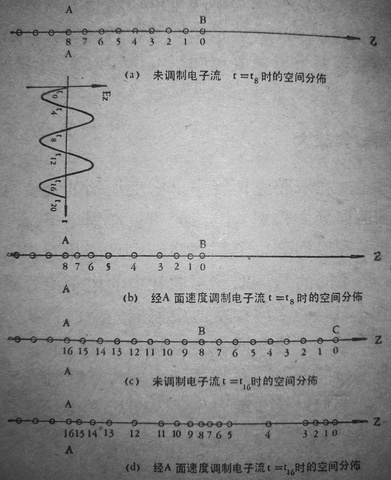
\includegraphics[width=0.8\linewidth]{figure/ch2-3}
	\caption{群聚电子流的形成}
	\label{ch2-3}
\end{figure}

下面,我们来看看经过两个调制电场周期后(即$ t=16 $时)电子的空间分布情况,如图\ref{ch2-3}(d)所示。由图可见,第一个周期内进入A-A面的那些电子,“两极分化”的程度变得更为严重,空间分布更加不均匀。不难想象,如果电子在漂移空间的这种惯性运动继续进行下去,那么,“两级分化”现象就会越来越严重,最后电子流变成一群一群或者一团一团的了。

从图\ref{ch2-3}我们可以看到,电子流中的电子是分别向0号、8号、16号$ \cdots $等电子靠拢的,这些电子就叫做“群聚中心”,这些电子有一个共同的特点:它们都是当调制电场$ E_z $由正半周变为负半周穿过零点的那些时刻进入A-A面的。由图可见,群聚电子流的密度将在这些“群聚中心”附近达到最大,因此,群聚电子流的密度调制频率是和调制电场$ E_z $的频率一致的。

现在,我们再回到行波管来。我们知道,在行波管中,始终有一个同步高频场随着电子流一起前进,那么,读者要问:同步高频场的存在会对电子流的群聚产生什么影响呢?是加强了群聚还是破坏了群聚?反过来,群聚电子流又是如何作用于同步高频场的呢?是把自己的能量交给高频场还是从高频场中得到能量?对于这两个问题的简要回答是:由于电子流与高频场是同步前进的,因此它们之间就可以持续地相互作用,互相得到加强:在同步高频电场的作用下,电子流的群聚不断得到加强;反过来,群聚电子流又不断地把自己的能量交给高频电场,使它增强。它们共同增长的结果就是在输出端处得到了比输入信号强得多的信号,这样,输入信号便得到了放大,这就是行波管的放大原理。我们把行波管内电子流密度和高频电场共同增长的情况形象地画在图\ref{ch2-4}中。
\begin{figure}[htbp]
	\centering
	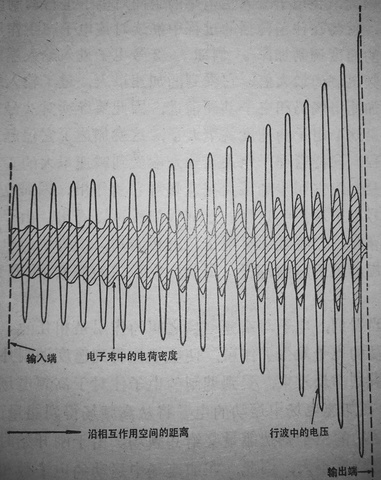
\includegraphics[width=0.7\linewidth]{figure/ch2-4}
	\caption{信号电压和群聚沿行波管相互作用而增长的情况}
	\label{ch2-4}
\end{figure}

下面,我们来比较详细地分析一下行波管内电子流与行波高频场相互作用的情况,以回答前面所提出的问题。

当均匀电子注进入螺旋线时,输入端处的高频电场就要对电子注进行速度调制。由于输入端的高频电场比较弱,因此电子注受到的速度调制是不大的。这些具有初步速度调制的电子注在继续向前运动的过程中将会受到螺旋线上高频电场的作用。图\ref{ch2-5}就表示了高频电场对电子流群聚的作用。图中画出了有同步高频电场存在时某两个时刻电子的空间分布图。和前面一样,我们规定$ E_z $的正方向与$ Z $轴的正方向相同,因此,对电子来说,$ E_z $为负时是加速场,$ E_z $为正时是减速场。在同步情况下,在输入端对电子进行初步速度调制的高频电场将与被调制的电子以相同的速度向前移动,它们之间处于相对静止状态。因此,在电子进入输入端的瞬间对电子进行调制的那个高频场,就将在往前传播的过程中继续对该电子产生作用,使得电子的速度调制加深。例如:2号电子进入输入端时正好碰上高频电场的最大值,它受到的加速最大,过了输入端后此最大加速电场仍和电子共同前进,因此要继续对2号电子加速,结果这个电子的速度就更大了,这就加速了它追赶0号电子的过程。同样道理,原来在输入端受到减速最大的6号电子将继续受到跟它同步的最大减速场对它的作用,因而也加速了它向8号电子靠拢的过程。这样我们就可以看出,由于同步高频场的存在,它将继续对电子注进行调制,使得快的电子越跑越快,慢的电子越跑越慢,因此,电子注的群聚便得到了加强。
\begin{figure}[phtb]
	\centering
	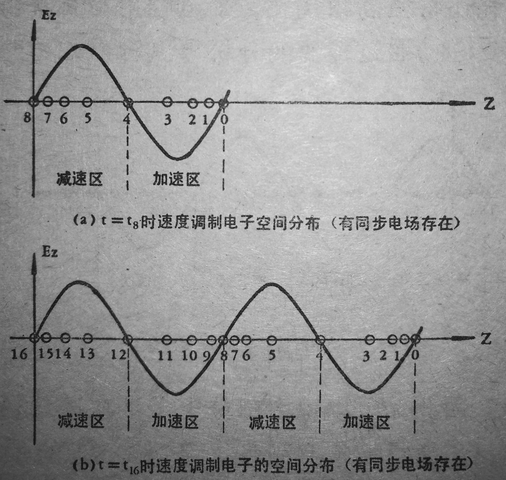
\includegraphics[width=0.65\linewidth]{figure/ch2-5}
	\caption{同步高频电场加强了电子流的群聚}
	\label{ch2-5}
\end{figure}

应当看到,电子与高频电场之间的作用是相互的。高频电场对运动的电子发生了作用,使电子注得到速度调制并逐渐变为密度调制;反过来,受到调制的电子注对于高频电场也要发生作用,在加速电场中运动的电子将从高频场得到能量,而在减速场中运动的电子则把能量交给高频场。由于刚开始时,电子注的群聚程度不大,因此,在加速场中运动的电子数和在减速场中运动的电子数基本上是相等的,总的效果是电子注和高颜场之间没有什么净能量交换。但是,当电子注和同步高频继续向前移动时,情况就不同了。从图\ref{ch2-5}(b)中我们可以看到,电子是向0号、8号、16号这样一些“群聚中心”电子掌拢的。因此,我们只要看看群聚中心的电子是在哪种性质的高频场中运动就可以知道总的能量交换是哪一方面占优势了。如前所述,群聚中心都是高频电场从减速场转为加速场穿过零点这一瞬间进入输入端的那些电子。那么,这些电子将在什么性质的高频场中运动呢?下面,我们来讨论几种情况:
\begin{enumerate}
	\item 假定电子注速度的直流分量是$ v_0 $,高频场的轴向传播速度为$ v_p $,如果两者完全相等,那么群聚中心就始终在零场中运动,群聚的电子群中有一半电子在加速场中运动,另一半在减速场中运动。因此,虽然电子注已经群聚,但由于群聚中心在零场中运动,总的效果,电子注和高频场之间仍然没有什么净能量交换。
	\item 如果电子的速度比高频场的传播速度略慢(即$ v_0 \leq v_p $),从图\ref{ch2-6}可以清楚地看出,群聚中心将落入加速场中,也就是说大部分电子将在加速场中运动,从高频场中吸收能量。总的效果是高频场把能量交给电子注,它本身不但得不到放大,反而迅速地衰减下来。
	\item 当电子速度和高频场传播速度相差很大(即$ v_0\gg v_p $或$ v_0 \ll v_p $)时,进入螺旋线的电子注一会儿受到加速场的作用一会儿受到减速场的作用,因而不可能得到有效的群聚,也就不能与高频场发生有效的能量交换。相反,由于螺旋线本身的损耗还将使高频场在传播过程中不断减弱。
	\item 通过前面的分析可以看出,如果要让群聚中心的电子在减速场中运动,就需要使电子注速度$ v_0 $比高频场的轴向传播速度$ v_p $稍快一些。这时的情况就象图\ref{ch2-7}所画的那样,由于群聚群聚中心已经落入减速场中,因此,可以说大部分电子是在减速场中运动的,它们将把自己的能量交给高频场。于是,总的看来,电子就有净能量交给高频场,使高频场增强。由于电子注和高频场始终是同步前进的,因此,这种能量交换是持续不断的。在电子注向前流动的过程中,螺旋线上的高频场不断对它作用,使得它的群聚不断加强;同时,加强了的群聚电子注又不断地把能量交给高频场,使得高频场不断地得到增强。最终,高频场就能得到可观的放大。我们把这个过程形象地用图\ref{ch2-8}表示出来。
\end{enumerate}

通过上面的讨论,我们可以看到:行波管是一种利用电子注与行波高频场之间持续的能量交换作用来放大微波信号的电子器件。由于螺旋线的频带很宽,因此,螺旋线型行波管的工作频带也很宽,这是它的一个很大的优点。行波管的另一个优点是增益高,这是因为在同步条件下,电子注与高频场能够持续地有效地发生能量交换的缘故。

\begin{figure}[phtb]
	\centering
	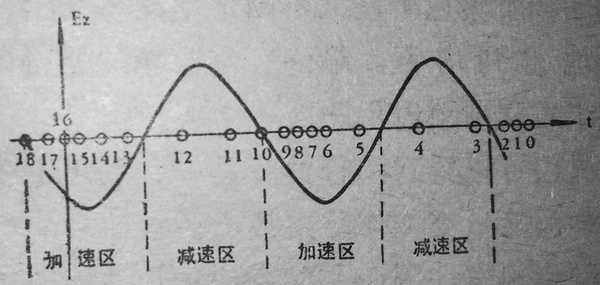
\includegraphics[width=0.6\linewidth]{figure/ch2-6}
	\caption{$ v_0 \leq v_p $时群聚中心落入加速场中}
	\label{ch2-6}
\end{figure}

\begin{figure}[phtb]
	\centering
	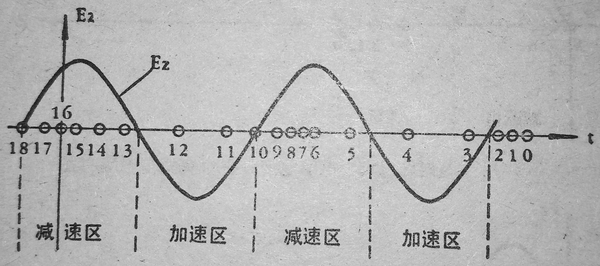
\includegraphics[width=0.6\linewidth]{figure/ch2-7}
	\caption{$ v_0 \geq v_p $时群聚中心落入减速场中}
	\label{ch2-7}
\end{figure}
\begin{figure}[phtb]
	\centering
	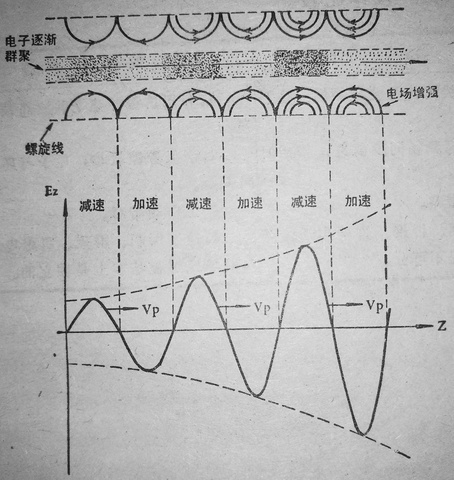
\includegraphics[width=0.65\linewidth]{figure/ch2-8}
	\caption{群聚电子流的形成}
	\label{ch2-8}
\end{figure}
从前面的分析中我们知道,所谓同步就是要使电子注的速度略大于高频场的传播速度,即$ v_0 \geq v_p $。这就是说,我们最初所建立的同步概念(即$ v_0 = v_p $)应当作一些修改。因为正如前面所分析的,当$ v_0 = v_p $时,交变电子流与高频电场之间将没有净能量交换。

在实际的行波管中,螺旋线的尺寸已经通过设计计算确定,也就是说,$ v_p $已经定了。那么,怎样使电子流和行波高频场达到“同步”呢?我们知道,电子的速度可以很方便地通过调节螺旋线电压来改变。因此,只要调节螺旋线电压$ U_H $便可以达到$ v_0 \geq v_p $的同步状态,此时,交变电子流能够最有效地把能量交给高频电场,使行波管的输出功率最大。可见,同步状态是与最大的输出功率相对应的,我们把此时的螺旋线电压叫做同步电压。通常,为了得到尽可能大的输出功率,人们总是把螺旋线电压调节到同步电压工作。

最后,让我们把行波管和双腔速调管的工作特点归纳一下,列成表\ref{tab:ch2-1},以作比较。

\begin{table} 
	\caption{行波管和双腔速调管的比较}\label{tab:ch2-1}
	\begin{tabular}{p{6cm}p{6cm}}
		\toprule
		\centering 行波管          &  \hspace{6em}双腔速调管    \\ \midrule
		\begin{enumerate}
			\item 用慢波线传输行波高频场,电场较弱。
			\item 电子与高频场同步前进,作用时时间长。
			\item 工作频带宽。
			\item 速度调制、群聚、群聚电子流激励高频场三过程不可分。
		\end{enumerate}	    & \begin{enumerate}
			\item 利用谐振腔建立驻波高频场,电场强。  
			\item 谐振腔隙缝小,电子与高频场作用间短。
			\item 工作频带窄。 
			\item 速度调制、群聚、群聚电子流激励高频场三过程基本上是独立的。
		\end{enumerate}	  \\ \bottomrule
	\end{tabular}
\end{table}
 

